\documentclass{book}

\usepackage[T1]{fontenc}
\usepackage{inconsolata}

\usepackage{color}
\definecolor{bluekeywords}{rgb}{0.13,0.13,1}
\definecolor{greencomments}{rgb}{0,0.5,0}
\definecolor{redstrings}{rgb}{0.9,0,0}
\usepackage{graphicx}
\graphicspath{ {images/} }
\usepackage{listings}
\lstset{language=[Sharp]C,
	frame=single,
	showspaces=false,
	showtabs=false,
	breaklines=true,
	showstringspaces=false,
	breakatwhitespace=true,
	escapeinside={(*@}{@*)},
	commentstyle=\color{greencomments},
	keywordstyle=\color{bluekeywords},
	stringstyle=\color{redstrings},
	basicstyle=\ttfamily
}

\definecolor{gray}{rgb}{0.4,0.4,0.4}
\definecolor{darkblue}{rgb}{0.0,0.0,0.6}
\definecolor{cyan}{rgb}{0.0,0.6,0.6}

\lstset{
	frame=single,
	basicstyle=\ttfamily,
	columns=fullflexible,
	showstringspaces=false,
	commentstyle=\color{gray}\upshape
}

\lstdefinelanguage{XML}
{
	frame=single,
	morestring=[b]",
	morestring=[s]{>}{<},
	morecomment=[s]{<?}{?>},
	stringstyle=\color{black},
	identifierstyle=\color{darkblue},
	keywordstyle=\color{cyan},
	morekeywords={xmlns,version,type}% list your attributes here
}

\begin{document}

\author{BlackCentipede}
\title{Platform Invocation Indepth\\
	   \large Licensed Attribution-NonCommercial-NoDerivs 2.5\\
   	   \small https://creativecommons.org/licenses/by-nc-nd/2.5/legalcode}
\date{November 2017}

\frontmatter
\maketitle
\tableofcontents

\mainmatter
\chapter{Introduction}
\section{What you will need to get started}
You will need Dotnet Core and Clang/LLVM compilers installed for this book. The book will assume you are working on Linux platform although knowledge gained here can be applied on any other platforms including Windows.

You can install Dotnet Core SDK from this URL: https://www.microsoft.com/net/download/linux
Clang/LLVM Compilers can be installed or compiled on your respective linux distribution.

\textbf{TODO}: Expound instructions for this part.

The book will be using Visual Studio Code IDE and CodeLite IDE.

\section{Minimum Knowledge}
You'll need to have some comprehension of C\# and C languages before starting this book.

\chapter{Introduction to P/Invoke}

\section{Getting Started}
First, create a Directory as 'ChapterTwo' for this project and create a new file, 'ChapTwo.c' under 'ChapterTwo' folder.

Let's assume we have a basic Addition function in a C Library that we want to call.

\begin{lstlisting}{c}
int Sum(int a, int b)
{
  return a+b;
}
\end{lstlisting}

It's a simple Addition Operation at a first glance, but there are\newline considerations that must be observed first before attempting to write platform invocation wrapper code for the function above:

\begin{enumerate}
	\item \label{itm:first} `int` datatype in C can be considered 2 bytes long or 4 bytes long or however long it may be depending on the architecture and compiler that the library is compiled on. In C Standard, int must be capable of containing \textbf{at least} the [\textminus32,767, +32,767] range; thus, it is at least 16 bits in size.
	
	\item Due to \ref{itm:first}, you can reasonably safeguard against data loss by substituting C\# Int32(int) which contains 4 bytes or you may choose follow the standard strictly by supplying C\# Int16(short) which contains 2 bytes, even though it can suffer data loss. The best approach is to avoid using "at least" integers in C and instead use fixed size integers provided by the compiler in ''stdint.h'' header if you have Foreign Function Interface kept in mind.
	
	\item Sometimes you have to keep Endianess in mind although it is less of a concern in x86\_64 architecture since little endianess is the default.
\end{enumerate}
\newpage
The best approach to writing the Addition function is to make it clear what sized integers you're attempting to add  if possible.

\begin{lstlisting}{c}
#include <stdint.h>
int32_t Sum(int32_t a, int32_t b)
{
  return a+b;
}
\end{lstlisting}

\section{Compiling the Library}
This book assumes you have sufficient knowledge of C, we will still however, provide compilation instruction. The following command assumes that you have named your source code file as 'ChapTwo.c' as instructed at the beginning of this chapter.

\begin{lstlisting}
clang -std=c99 -shared -fPIC -olibChapTwo.so ChapTwo.c
\end{lstlisting}

Here we examine and explain the compiler arguments:

\begin{enumerate}
	\item '-std=c99' specify that we are compiling C source code under C99 Standard.
	\item '-shared' specify that we want the program to be compiled as shared/dynamic library.
	\item '-fPIC' specify that code must be position independent so that the resultant library can be loaded by other processes and have code be made available to be run anywhere in program address space regardless of code's address.
	\item '-olibChapTwo.so' specify what the output library should be named. lib prefix in 'libChapTwo.so' is a matter of naming convention to be followed on Linux although compilers like clang and gcc do search libraries based on lib prefix when using '-l' option. 
\end{enumerate}
\newpage
\section{Configuring C\# Project}
Since we're already in "ChapterTwo" directory, we can go ahead and run 'dotnet new Console'. There are a few steps we need to take to add the C code to our C\# project. First, we need to automate the compilation process of our C file and copy the compiled C library to the target directory for Debug, Release, or any other configurations.

Open up 'ChapterTwo.csproj' file with your favorite editor, and add the following under '</PropertyGroup>' inside '<Project>' tag.

\begin{lstlisting}{language=XML}
<Target Name="CompileCProject" AfterTargets="AfterBuild">
	<exec Command=
	"clang -std=c99 -shared -fPIC -olibChapTwo.so
	ChapTwo.c" />
	<Copy SourceFiles="libChapTwo.so" DestinationFolder="$(OutDir)" />
</Target>
\end{lstlisting}

The snippet above does few things after building our C\# project:
\begin{enumerate}
	\item Compile ChapTwo.c code as a shared library, libChapTwo.so
	\item Copy libChapTwo.so into any target directory that C\# is being built in.
\end{enumerate}

This makes it significantly easier to modify our code without having to run any additional commands for it to take effect.

Your CSProj should look like the following:

\begin{lstlisting}{language=XML}
<Project Sdk="Microsoft.NET.Sdk">

 <PropertyGroup>
  <OutputType>Exe</OutputType>
  <TargetFramework>netcoreapp2.0</TargetFramework>
 </PropertyGroup>
 <Target Name="CompileCProject" AfterTargets="AfterBuild">
  <exec Command="clang -std=c99 -shared -fPIC -olibChapTwo.so
ChapTwo.c" />
  <Copy SourceFiles="libChapTwo.so" DestinationFolder="$(OutDir)" />
 </Target>
</Project>
\end{lstlisting}
\newpage
\section{Wrapping C Code in C\#}
Open up Program.cs, add a new using directive at the top of your source code.

\begin{lstlisting}{c}
using System.Runtime.InteropServices;
\end{lstlisting}

This line imports all of the platform invocation services which enables us to interact with our C library with ease.

Add the following lines under Program class:

\begin{lstlisting}{c}
[DllImport("ChapTwo")]
static extern int Add(int a, int b);
\end{lstlisting}

The DllImport attribute declares that a static externally defined function is defined in a C library and to have CLR create a Platform Invocation stub to define the said function within external library.

It is required to declare the function with static and extern modifiers since it is a function that is both independent of state and externally defined.

Finally, modify the ''Console.WriteLine'' line to the following:

\begin{lstlisting}{c}
Console.WriteLine("1 + 2 = {0}", Add(1, 2)};
\end{lstlisting}
And your source code should look as follows:

\begin{lstlisting}{c}
using System;
using System.Runtime.InteropServices;
namespace ChapterTwo
{
	class Program
	{
		[DllImport("ChapTwo")]
		static extern int Add(int a, int b);
		static void Main(string[] args)
		{
		Console.WriteLine("1 + 2 = {0}", Add(1, 2));
		}
	}
}
\end{lstlisting}
\newpage
Finally, your program is ready to be executed. You can run:

''dotnet restore \&\& dotnet run''

And we have the following:

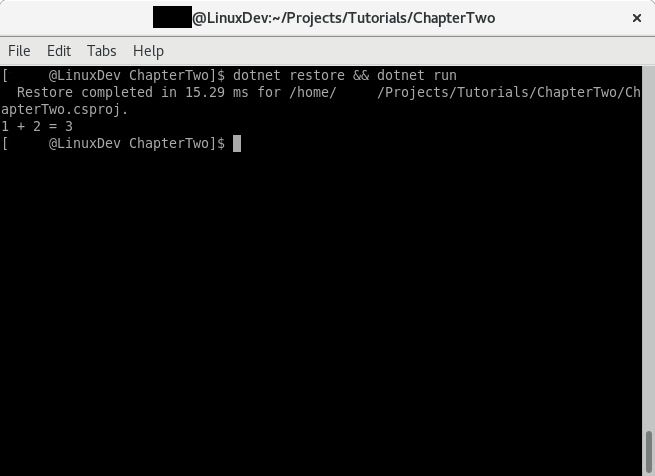
\includegraphics[width=\textwidth]{ChapTwoConsole}
It works as expected!
\newpage
\section{Some background}
There are few things happening when a function with DllImport is called, if this is the first time the function is being called, the Runtime will first load the external library immediately, then load the symbol ''Add'' by default, and finally generate a P/Invoke stub for that function to support the call to the external function.

The symbol is merely just that, a symbol that is exported by C Library. You can find a list of symbols by running ''objdump -T libChapTwo.so'' on your library and you'll have the following:

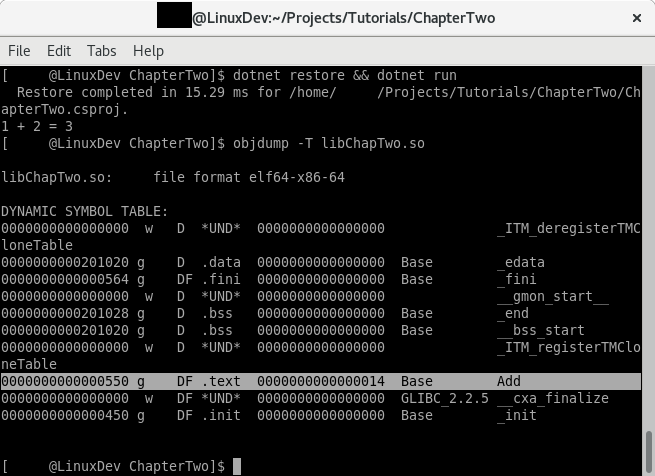
\includegraphics[width=\textwidth]{ChapTwoConsoleTwo}

You will notice that the Add symbol is shown in the symbol table in your library, this is how the CLR looks up a function by entry name.
\chapter{Introduction to Pointer}
\section{Overview on Pointer}
If you already have sufficient understanding about Pointer in both C\# and C languages, you can skip this chapter. This chapter is for introducing beginners to the concept of pointer.

A pointer is essentially an address to an area of memory. You can represent what that pointer is supposed to be such as a pointer of integer, struct, classes, function or even another pointer.
To read and write memory that pointer is pointing to, you have to first dereference that pointer and you can do so by using asterisk in front of a pointer variable to dereference it, not to be confused with multiplication operator.

\begin{lstlisting}{c}
#include <stdlib.h>
#include <stdint.h>

int32_t* MyPointer = (int32_t*)malloc(sizeof(int32_t));

// You can access pointer like an array
MyPointer[0] = 12;

// You can also dereference a pointer to read or write the data in memory directly.
*MyPointer = 12;
\end{lstlisting}

The C snippet above first allocate with malloc function a new buffer of memory up to a size of int32\_t datatype and return a void* pointer which then get casted into int32\_t* pointer type. You can access the pointer in two ways, writing it similar fashion as you would when accessing an array and to use '*' operator to dereference the pointer to read and write the first datatype the pointer is currently pointing to.
\newpage
Let's get started by creating a new "ChapterThree" directory and create a new file, "ChapThree.c" and open with your favorite editor.

We will need three headers to provide the functionalties and types we need for this chapter.

\begin{lstlisting}{c}
#include <stdlib.h> // For malloc function
#include <stdio.h> // for printf function
#include <stdint.h> // for int32_t type
\end{lstlisting}

Let's declare a main function that allocate a buffer of 20 integers and return a pointer address to that buffer and we'll treat it as an array of integer.

\begin{lstlisting}
int main()
{
	int32_t* buffer = (int32_t*)malloc(sizeof(int32_t)*20);
	// Let's do some math on our buffer!
	for (int32_t I = 0; I < 20; ++I)
	{
		buffer[I] = I * 2;
	}
	
	// Now let's print what our buffer is going to look like:
	for (int32_t I = 0; I < 20; ++I)
	{
		printf("Buffer[%i] = %i\n", I, buffer[I]);
	}
	
	free(buffer);
}
\end{lstlisting}
\newpage
The output would be shown as this:

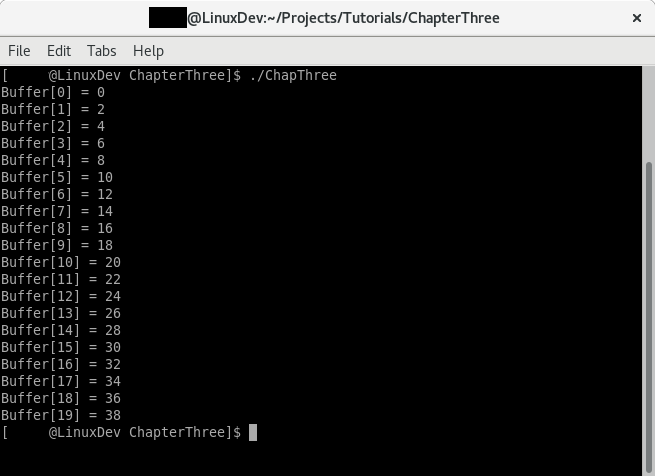
\includegraphics[width=\textwidth]{ChapThreeConsole}

There are few things that may be confusing in the snippet above and why it is an acceptable practice in C:

\begin{enumerate}
	\item When you use malloc to allocate buffer, malloc keeps a record of how big the block of memory is so that it can be freed in later time, however you cannot and should not access that size information within malloc, keeping track of buffer size is your responsibility.
	
	\item When using malloc, you allocate the amount of data you would need by using sizeof keyword to determine how many bytes capacity you need in a buffer to cover that information and you can multiply that element size by the number of elements you want allocated for your program. In the snippet above, size of int32\_t type would resolves to 4 and then multiplied by 20, so we would have a buffer that have the capacity to hold 20 int32\_t elements.
\end{enumerate}

Because of the fact behind malloc/free that LibC does store information about the pointer that is allocated with those functions, it discouraged to use different library or framework to free that memory, although most library and framework may likely use the same functions.
\newpage
\section{The Function Pointers}
Function pointers are a bit of a tongue twister, because the way it is defined in C can be confusing.

\begin{lstlisting}
int32_t (*Add)(int32_t, int32_t);
\end{lstlisting}

The snippet above is a declaration of function pointer for a function that returns a int32\_t after accepting two int32\_t parameters. It currently pointing at nothing and would cause segmentation fault when you attempt to call it, so you have to assign a function for it to be used.

One example of this use case is that we can dynamically modify the behavior of our program during runtime and essentially allow our program to switch logic at different points during program execution like so:
\begin{lstlisting}
#include <stdlib.h>
#include <stdio.h>
#include <stdint.h>

int32_t (*Add)(int32_t, int32_t);

int32_t ActualAddingFunction(int32_t a, int32_t b)
{
	return a + b;
}

int32_t FalseAddingFunction(int32_t a, int32_t b)
{
	return a - b;
}

int main()
{
	int A = 1;
	int B = 2;
	
	Add = ActualAddingFunction;
	
	printf("Let's try ActualAddingFunction: %i\n", Add(A, B));
	
	Add = FalseAddingFunction;
	
	printf("Let's try FalseAddingFunction: %i\n", Add(A, B));
}
\end{lstlisting}
\newpage
It would produce an output as followed:

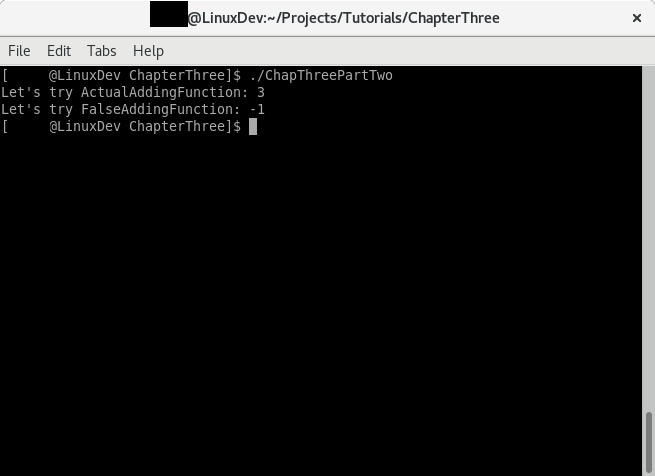
\includegraphics[width=\textwidth]{ChapThreeConsoleTwo}
\newpage
\section{C\# Counterpart}
C\# does support pointer so long that the code blocks, methods, or types are defined with unsafe modifier. Those can be accomplished by using snippets below as a demonstration:
\begin{lstlisting}{c}
public unsafe void DoBufferAllocation()
{
	int* MyIntegerPointer = (int*)Marshal
		.AllocHGlobal(Marshal.SizeOf<int>()).ToPointer();
	
	// You can use it in a similar fashion as you would in C.
	*MyIntegerPointer = 123;
}
\end{lstlisting}

\begin{lstlisting}{c}
public unsafe class Demo {
	public void DoBufferAllocation()
	{
		int* MyIntegerPointer = (int*)Marshal
		.AllocHGlobal(Marshal.SizeOf<int>()).ToPointer();
		
		*MyIntegerPointer = 123;
	}
}
\end{lstlisting}

\begin{lstlisting}{c}
public void DoBufferAllocation()
{
	unsafe {
		int* MyIntegerPointer = (int*)Marshal
		.AllocHGlobal(Marshal.SizeOf<int>()).ToPointer();
		
		*MyIntegerPointer = 123;
	}
}
\end{lstlisting}

However, compiler will throw an error unless you explicitly specify that you want to compile unsafe code. For CoreCLR, you can do so by adding the following into your csproj file inside the  <PropertyGroup> tags:

\begin{lstlisting}{xml}
<AllowUnsafeBlocks>true</AllowUnsafeBlocks>
\end{lstlisting}
\newpage
Marshal static class from System.Runtime.InteropServices offer a variety of functions for marshaling pointers to usable data types and vice versa. You can also generate a function in runtime in CLR and pass it over to C program so that C program can use your newly created function during it's execution.

\textbf{TODO}: Add project to demonstrate the above.
\chapter{Externally Defined Variables}
\section{Moving Forward}
Let's create a new directory for this chapter, name it ''ChapterFour''. As the chapter implied, we now want to access variables that are defined in C Library, but unfortunately, C\# does not offer an easy approach to accomplish this, so we must look into Marshal static class that is provided in\newline ''System.Runtime.InteropServices'' namespace.

Let's create a new C source code file, ''ChapFour.c'' and open it with your favorite editor.

Add the following code to your source code:

\begin{lstlisting}{language=c}
#include <stdint.h>

int32_t MyVariable = 123;

void ResetMyVariable()
{
	MyVariable = 123;
}
\end{lstlisting}

You can compile the following code by running this command:

\begin{lstlisting}
clang -std=c99 -shared -fPIC -olibChapFour.so ChapFour.c
\end{lstlisting}
\newpage
You can export a list of symbols by running 
\begin{lstlisting}
objdump -T libChapFour.so
\end{lstlisting}

You will notice that we have a symbol for ''MyVariable''.

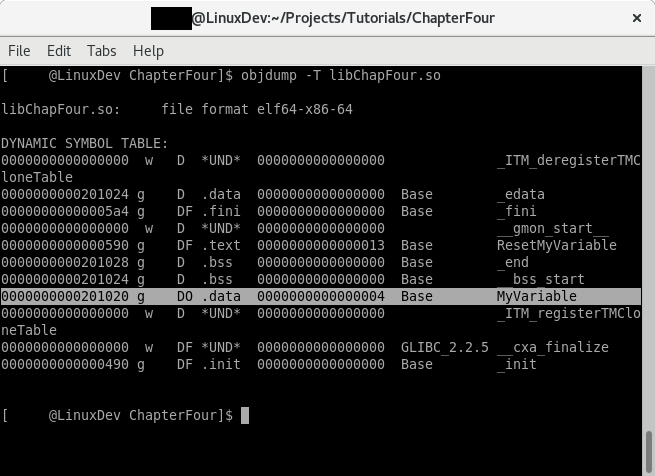
\includegraphics[width=\textwidth]{ChapFourConsole}

\section{Loading the Library Dynamically}
As mentioned above, we cannot normally access library that is loaded by the CLR already directly. In Mono Runtime, it will use DL library to load the library only once in this method, but \textbf{CoreCLR as of this time of writing (Nov 24, 2017) will load entirely new instance of library apart from DL library approach.}

Both DL library (for Linux Platform) and Kernel32.dll(Windows Platform) provide functions to load library and to return a handle for the same library if it is already previously loaded and haven't been freed first.

For the course of this chapter, we will load 3 new functions from DL library in order to enable us to access library that may already be loaded, dlopen, dlsym, and dlclose functions.

Let's get started by running the following command:

\begin{lstlisting}
dotnet new Console
\end{lstlisting}
\newpage
Open up ''ChapterFour.csproj'' file and add the following snippet under </PropertyGroup> tag inside <Project> tags.

\begin{lstlisting}{language=XML}
<Target Name="CompileCProject" AfterTargets="AfterBuild">
  <exec Command=
  "clang -std=c99 -shared -fPIC -olibChapFour.so
ChapFour.c" />
  <Copy SourceFiles="libChapFour.so" DestinationFolder="$(OutDir)" />
</Target>
\end{lstlisting}

Add the following line in <PropertyGroup> tags:

\begin{lstlisting}
<AllowUnsafeBlocks>true</AllowUnsafeBlocks>
\end{lstlisting}

Your ChapterFour.csproj should look like the following:

\begin{lstlisting}
<Project Sdk="Microsoft.NET.Sdk">

 <PropertyGroup>
  <OutputType>Exe</OutputType>
  <TargetFramework>netcoreapp2.0</TargetFramework>
  <AllowUnsafeBlocks>true</AllowUnsafeBlocks>
 </PropertyGroup>
 <Target Name="CompileCProject" AfterTargets="AfterBuild">
  <exec Command="clang -std=c99 -shared -fPIC -olibChapFour.so
ChapFour.c" />
  <Copy SourceFiles="libChapFour.so" DestinationFolder="$(OutDir)" />
 </Target>
</Project>
\end{lstlisting}
Now open ''Program.cs'' source code file and append the using directive at the top of the source code:

\begin{lstlisting}{language=c}
using System.Runtime.InteropServices;
\end{lstlisting}
\newpage
Now we need to load the externally defined functions for dynamically loading a library and to load the reset function from ''libChapThree.so'' library. Append the following codes inside Program class:

\begin{lstlisting}{language=c}
[DllImport("dl")]
static extern IntPtr dlopen(string file, int flag = 1);

[DllImport("dl")]
static extern IntPtr dlsym(IntPtr handle, string symbol);

[DllImport("dl")]
static extern int dlclose(IntPtr handle);

[DllImport("ChapFour")]
static extern void ResetMyVariable();

delegate void ResetMyVariable_dt();
\end{lstlisting}

Finally replace Main method with the following snippet:

\begin{lstlisting}
static unsafe void Main(string[] args)
{
	var libPath = "./libChapFour.so";
	IntPtr libraryHandle = dlopen(libPath);
	int* ptr = (int*)dlsym(libraryHandle, "MyVariable").ToPointer();
	Console.WriteLine("MyVariable Value: {0}", *ptr);
	
	*ptr = *ptr + 1;
	Console.WriteLine("Incremented Variable: {0}", *ptr);
	
	ResetMyVariable();
	Console.WriteLine("MyVariable after CLR Loaded ResetMyVariable Execution: {0}", *ptr);
	
	var resetVariable = Marshal.GetDelegateForFunctionPointer<ResetMyVariable_dt>
		(dlsym(libraryHandle, "ResetMyVariable"));
	resetVariable();
	Console.WriteLine("MyVariable after DL Loaded ResetMyVariable Execution: {0}", *ptr);
	
	dlclose(libraryHandle);
}

\end{lstlisting}
\newpage
There are few things happening here:

\begin{enumerate}
	\item ResetMyVariable\_dt is a delegate type declaration to convert a simple function pointer to a usable function in C\#. The \_dt suffix is acronym for delegate type.
	\item The optional parameter, flag, in dlopen function is default to RTLD\_LAZY flag which is 0x00001.
	\item Method must be marked as Unsafe whenever pointer datatype such as ''int*'' is used.
	\item Library Path is simply a path to the library that is in the current directory.
	\item The dlsym returns a pointer to the variable which then can be interacted with in C\# program and C library.
	\item When running this code in Mono and Dotnet Core, the result will be drastically different from one another. Mono will load the library only once and share the same handle while Dotnet core would create 2 different instances of the same library and therefore data that is defined in each library will not match.
\end{enumerate}

\newpage
Your source code for Program.cs should look like below:
\begin{lstlisting}{c}
using System;
using System.Runtime.InteropServices;

namespace ChapterFour
{
	class Program
	{
		[DllImport("dl")]
		static extern IntPtr dlopen(string file, int flag = 1);
		
		[DllImport("dl")]
		static extern IntPtr dlsym(IntPtr handle, string symbol);
		
		[DllImport("dl")]
		static extern int dlclose(IntPtr handle);
		
		[DllImport("ChapFour")]
		static extern void ResetMyVariable();
		
		delegate void ResetMyVariable_dt();
\end{lstlisting}
\newpage
\begin{lstlisting}{c}
		static unsafe void Main(string[] args)
		{
			var libPath = "./libChapFour.so";
			IntPtr libraryHandle = dlopen(libPath);
			int* ptr = (int*)dlsym(libraryHandle, "MyVariable").ToPointer();
			Console.WriteLine("MyVariable Value: {0}", *ptr);
			*ptr = *ptr + 1;
			Console.WriteLine("Incremented Variable: {0}", *ptr);
			ResetMyVariable();
			Console.WriteLine("MyVariable after CLR Loaded ResetMyVariable Execution: {0}", *ptr);
			var resetVariable = Marshal
				.GetDelegateForFunctionPointer
				<ResetMyVariable_dt>
				(dlsym(libraryHandle, "ResetMyVariable"));
			resetVariable();
			Console.WriteLine("MyVariable after DL Loaded ResetMyVariable Execution: {0}", *ptr);
			dlclose(libraryHandle);
		}
	}
}
\end{lstlisting}
\newpage
In dotnet core, we have the following:

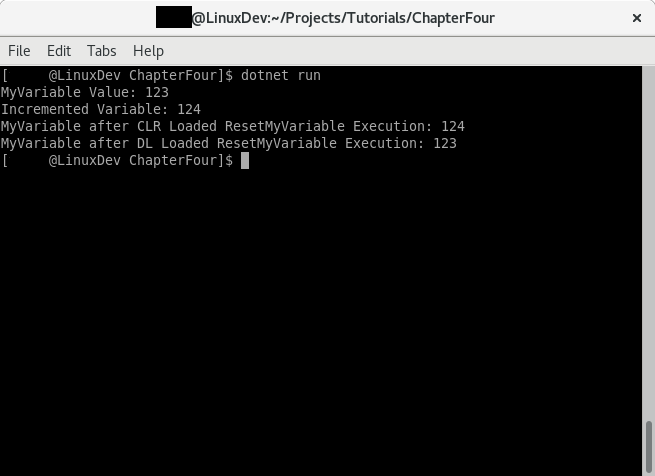
\includegraphics[width=\textwidth]{ChapFourConsoleOutputCore}

In Mono, we have the following:

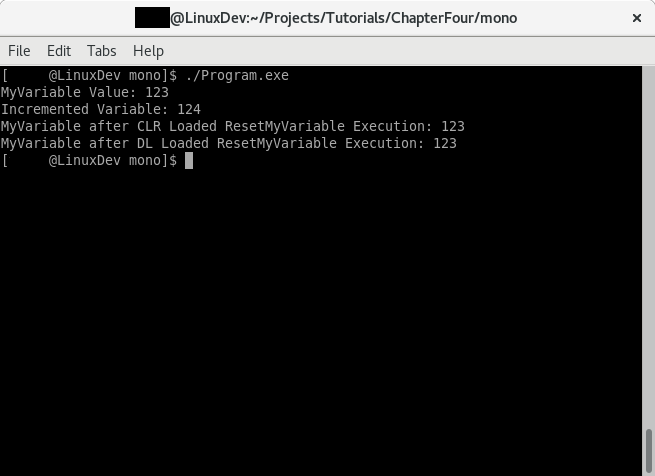
\includegraphics[width=\textwidth]{ChapFourConsoleOutputMono}
\newpage
\section{The Delegate Approach}
The difference is highlighted and as you can see, the result can be drastically different from one another and the behavior you see and expect in Dotnet Framework \textbf{WILL NOT} be consistent.
There is a different approach to tackle this particular issue.
We can limit our use of P/Invoke services provided by CLR to just loading DL library itself.
We can use DL library to load all externally defined functions and symbols within C\# and keep result and behavior consistent as demonstrated in both consoles above on the DL Loaded ResetMyVariable Execution line.
This approach is refered as the Delegate Approach.

\textbf{TODO}: Add Delegate Stub and Project to demonstrate how to work around the issue described above.
\backmatter
% bibliography, glossary and index would go here.

\end{document}